%% This is file `elsarticle-template-1-num.tex',
%%
%% Copyright 2009 Elsevier Ltd
%%
%% This file is part of the 'Elsarticle Bundle'.
%% ---------------------------------------------
%%
%% It may be distributed under the conditions of the LaTeX Project Public
%% License, either version 1.2 of this license or (at your option) any
%% later version.  The latest version of this license is in
%%    http://www.latex-project.org/lppl.txt
%% and version 1.2 or later is part of all distributions of LaTeX
%% version 1999/12/01 or later.
%%
%% Template article for Elsevier's document class `elsarticle'
%% with numbered style bibliographic references
%%
%% $Id: elsarticle-template-1-num.tex 149 2009-10-08 05:01:15Z rishi $
%% $URL: http://lenova.river-valley.com/svn/elsbst/trunk/elsarticle-template-1-num.tex $
%%
\documentclass[preprint,review,times,12pt]{elsarticle}

%% Use the option review to obtain double line spacing
%% \documentclass[preprint,review,12pt]{elsarticle}

%% Use the options 1p,twocolumn; 3p; 3p,twocolumn; 5p; or 5p,twocolumn
%% for a journal layout:
%% \documentclass[final,1p,times]{elsarticle}
%% \documentclass[final,1p,times,twocolumn]{elsarticle}
%% \documentclass[final,3p,times]{elsarticle}
%% \documentclass[final,3p,times,twocolumn]{elsarticle}
%% \documentclass[final,5p,times]{elsarticle}
%% \documentclass[final,5p,times,twocolumn]{elsarticle}


\usepackage[left=1in, right=1in, top=1in, bottom=1in]{geometry}
\usepackage{array}
\usepackage{multirow}
\usepackage{graphicx}
\usepackage{amssymb}
\usepackage{amsthm}
\usepackage{amsmath}
\usepackage{lineno}
\usepackage{setspace}
\usepackage{pdflscape}
\usepackage{natbib}

\journal{Ecography}
\setcitestyle{authoryear,round,semicolon,sort}
\bibliographystyle{apalike}
\begin{document}
\begin{frontmatter}

\title{Leveraging citizen science to assess richness, diversity, and abundance}

\author[DEE]{Tim M. Szewczyk}
\author[DEE]{Cleo Bertelsmeier}
\author[DEE]{Tanja Schwander}

\address[DEE]{Department of Ecology and Evolution, University of Lausanne}


\begin{abstract}
Abstract.
\end{abstract}

\begin{keyword}
Keywords
\end{keyword}

\end{frontmatter}
\linenumbers



\section{Introduction}
\label{S:1}
% Broad introduction: 
What structures ant species richness, diversity, and community structure at different spatial scales? We know that at a coarse scale, climate is generally important, with some support for phylogenetically conserved temperature preferences. At a local scale, richness typically decreases with canopy cover. In general, abundance seems to be more idiosyncratic and variable, both temporally and spatially. This is particularly true for small species. In ants, abundance can be measured as either the number of colonies in a particular area (i.e., colony density) or as the number of workers (i.e., worker density). 

Increasingly, ecologists have access to occurrence data collected in various and haphazard ways, typically in the form of online databases or citizen science projects (e.g., GBIF, BEIN, etc). These data are commonly used for species distribution models (CITE), including for individual species and hierarchical models of species communities \citep{Ovaskainen2017}, which can incorporate trait data, phylogeny, and covariation among species in addition to environmental drivers. However, they are a recent development and so far rely on a single set of occurrence data. However, use of such occurrence data for predicting richness or diversity directly has been somewhat more limited, though it is perhaps conceptually similar to extracting richness from guidebooks, which is fairly common (macroecology examples). There are several reasons for this. First, the data do not generally come from communities or assemblages, but rather an aggregation of detections from many different collectors across a variety of time spans. We like to think of diversity and richness as properties of communities, and these are decidedly not samples of communities, obscuring the ability to detect or account for interactions among species. Second, the collections for each species may have differing spatial biases, rendering any simple aggregation methods erroneous. Third, there are biases in the species that are more likely to be detected, such that any estimate of richness or diversity will necessarily be of a subset of the community biased toward larger, more active, or more interesting species.

However, that doesn't mean these data can't be useful. Instead, the geographic breadth and rather indiscriminate collection methods can capture occurrences in unexpected locations or detect species that may be missed in alternative, more structured sampling methods. Leveraging the widely available occurrence data could thus clarify patterns of species distributions and diversity, and the drivers that shape them.

Here, we combine species occurrences of ants collected in a citizen science project in western Switzerland with species abundance data from a concurrent structured sampling effort. In a hierarchical Bayesian framework, we use the citizen science data to help inform species' responses to regional variables, and the structured samples to inform responses to both regional and local variables, while accounting for bias in geographic and taxonomic sampling effort in the citizen science data. With this model, we detail the patterns of ant colony density and species diversity across the landscape while incorporating uncertainty in species compositions, and we evaluate the support for hypothesized drivers across spatial scales. We compare inferences from the combined model with those from each dataset independently, and also assess the differences in observed communities from each sampling method. 





\section{Methods}
\label{S:2}
\subsection{Study region \& sampling design}
This is a blurb about Vaud, including some about the climate, topography, as well as current and past human land use. Also a little bit about what is known about the ant fauna here, perhaps.


\begin{figure}
	\centering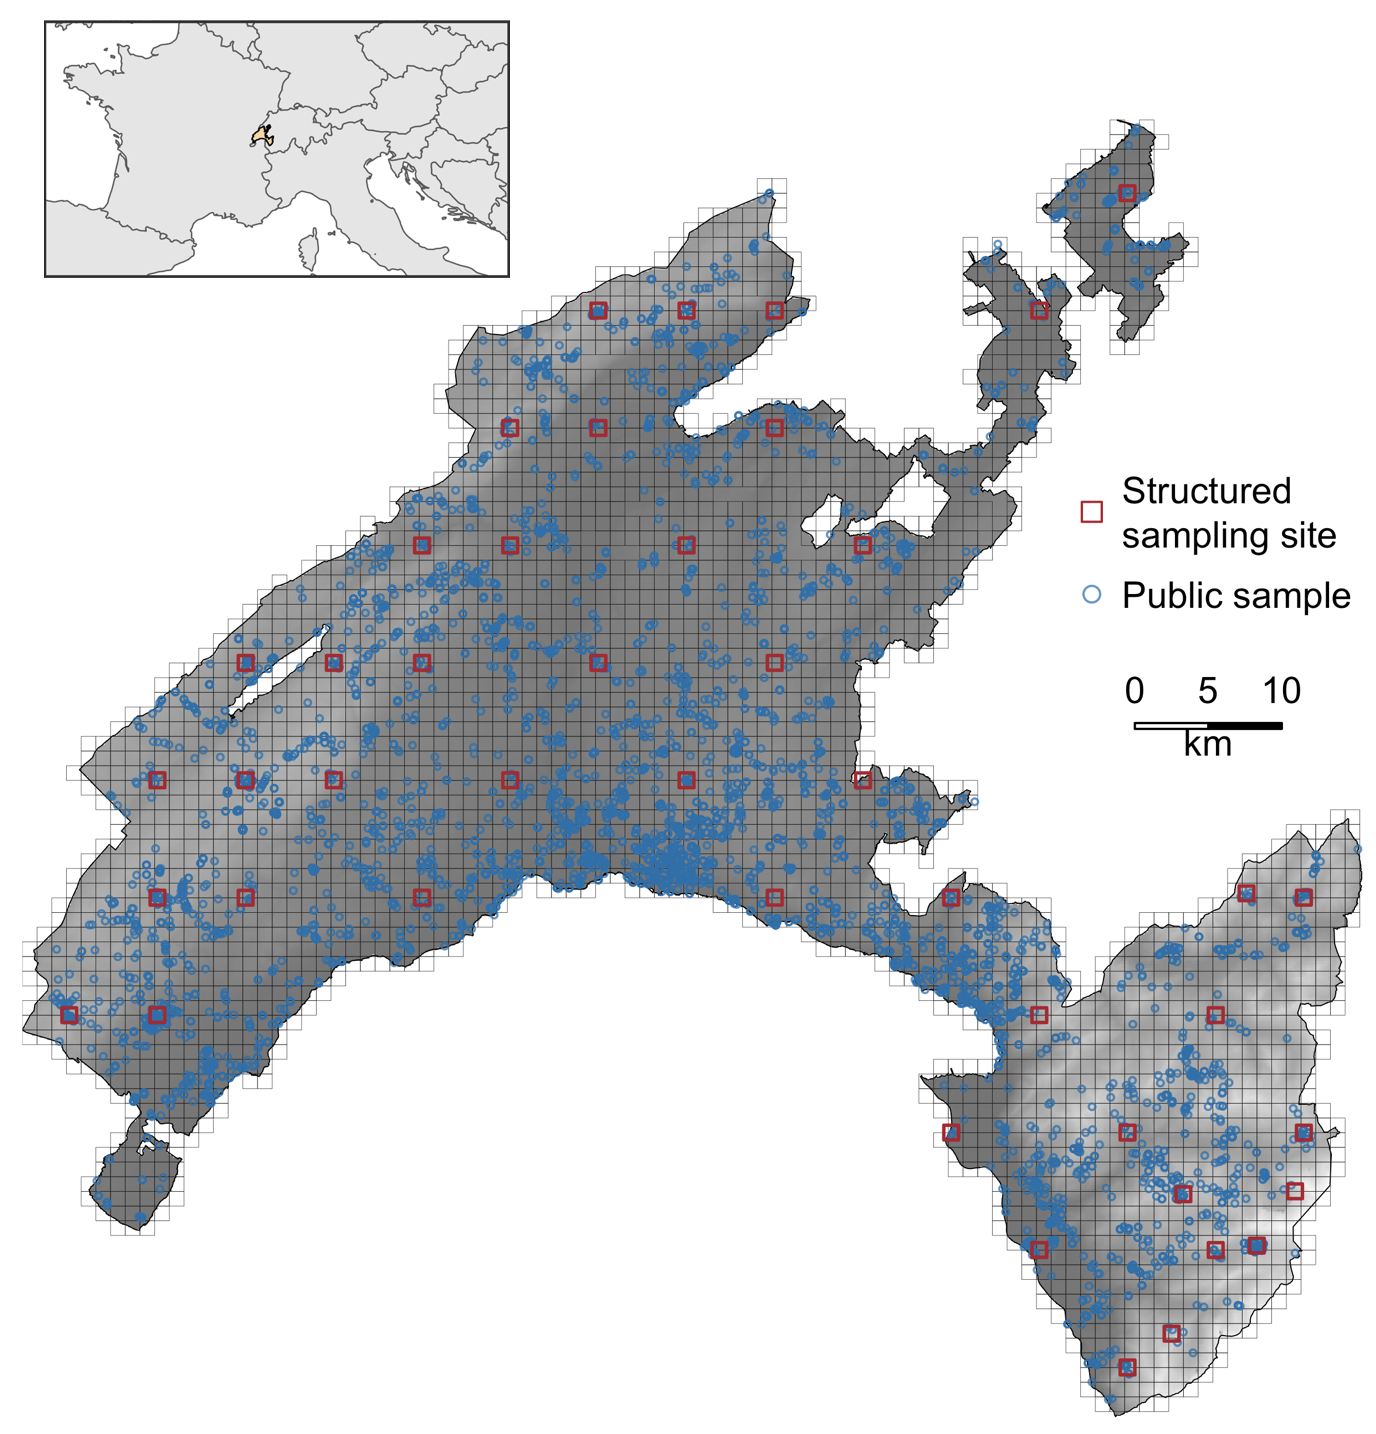
\includegraphics[width=3.5in]{figs/map_VD+inset.png}
	\caption{\label{fig:VD_map} Map of the canton of Vaud, Switzerland. Samples consisted of presence-only data (blue points) and structured abundance data collected at 1 km$^2$ long-term biodiversity monitoring sites (red squares). }
\end{figure}

% Methods for citizen science data
Ants were collected during the summer of 2019 in two simultaneous collection efforts (Fig. \ref{fig:VD_map}). First, a citizen science project (Opération Fourmis: https://wp.unil.ch/fourmisvaud/) was organized to survey the ant fauna within the canton of Vaud. Vials of ethanol were distributed to interested citizen scientists, who were asked to collect approximately 10 ant workers per colony for each vial. Participants were encouraged to explore under rocks, on bark, inside twigs, and in downed wood, and an online map was updated periodically to highlight data-sparse areas. Collectors returned the vials along with the collection date and the locality of the sample including the latitude and longitude. A total of TK samples were returned, representing collections between TK and TK. For these presence-only data, we discretized the landscape into a 1 km$^2$ grid (3,558 km$^2$) and tallied the number of counts for each species in each cell (TK cells with occurrences). 

% Methods for structured samples
Second, a structured sampling effort collected local colony abundance data, where ants were collected within 44 sites of 1 km$^2$ each, with standardized effort across sites. Thirty-nine of the sites were a part of long-term biodiversity monitoring efforts by the federal government, and as such were arranged on a regular grid with approximately 5-7 km between adjacent sites. Five additional sites are established monitoring sites by the University of Lausanne. The ants at each site were characterized by 25 plots, distributed among habitat types in approximate proportion to the abundance of each habitat, where each habitat type present within the site was represented by at least one plot. Inaccessible areas (e.g., cliffs, water, property beyond Vaud) were excluded, resulting in several sites with areas less than 1 km$^2$, and the number of plots was reduced proportionally (TK total plots; Appendix 1). 

Each sampling plot consisted of a 2m radius circle, with soil temperature recorded in the center at a depth of approximately 6 cm, and vegetation characterized according to Braun-Blanquet coverage classes (grass, forb, shrub, litter, bare, moss) within the plot (CITE). Six flags were evenly spaced around the circumference. Within $\sim$ 20 cm of each flag (total surface area $\sim$ 0.75 m$^2$), we searched for ant colonies within any downed wood or stumps, under large rocks, and in 2 L of soil, litter, and small rocks using 18 cm Hori Hori gardening knives. We haphazardly collected 10 workers from each colony, placing them directly into vials of ethanol. A total of TK colonies were detected across the 44 sites. Within each plot, all trees $\geq$3 cm diameter at breast height were also inspected for ant workers which were collected regardless of whether or not a colony was identifiable. Lastly, transect lines were mapped \emph{a priori}, distributed proportionally among habitat types and totalling 2 km, and surveyed at a moderate pace. Workers were collected from all permanent above-ground mounds within 2 m of the transect line. Because of the distinct sampling methods, the tree and transect collections were treated as presence-only data, and incorporated into the citizen science dataset (TK additional occurrences). 

Thus, each dataset has distinct strengths and limitations. The presence-only dataset was collected very broadly spatially, with a subset of detections resulting from free investigation of subjectively suitable habitats by skilled myrmecologists, and was therefore more likely to include rare or secretive species. However, many collections form citizen scientists occurred in or near human-dominant areas, with a likely bias toward larger, more obvious, or more anthropophilic species. The sampling effort also varied widely across space. In contrast, the structured abundance dataset was collected with uniform sampling effort, with a sampling design aimed to produce representative samples of colony density within each site. The communities from this dataset are thus expected to be more representative of the ground-nesting ant community structure, despite detecting a smaller number of species. 

% Identification and storage
All ants were identified to species or species group based on morphology by local experts (names?). Specimens are stored at the Natural History Museum of Lausanne in Lausanne, Switzerland in TK\% ethanol or mounted on pins. 


\subsection{Model overview}
To leverage the strengths of each dataset, we used a community-level hierarchical inhomogenous Poisson point process model (PPM). Inhomogenous Poisson PPMs assume that the distribution of occurrences is dependent on the variation in local intensity, $\lambda(x)$, across space, $x$, which may be observed imperfectly resulting in a thinned point process. One key benefit of PPMs is that the underlying latent intensity is continuous in space, and can be integrated to arbitrary spatial resolutions \citep{Baddeley2015,Hefley2016}. Following the structure of the sampling design, we modelled the expected intensity of each species at two resolutions (regional: 1 km$^2$, local: 0.75 $m^2$), representing the area of the sampling sites and the area of the sampling plots respectively. The modelled local intensities are a function of species' responses to the local and regional environment, with the structured abundance data incorporated at the local scale, and the presence-only data incorporated at the regional scale. 


\subsection{Model structure}
The hierarchical PPM unites the two datasets, $\textbf{W}$ (presence-only citizen science collections; resolution: 1 km$^2$) and $\textbf{Y}$ (structured local abundance collections; 0.75 $m^2$ plots within 1 km$^2$ sites). Thus, $\textbf{W}$ informs responses to regional environmental variables, and  $\textbf{Y}$ informs responses to both regional and local environmental variables. Similarly, $\textbf{W}$ helps to identify overall relative abundance among species, while $\textbf{Y}$ is a direct measurement of local abundance. We assume that local colony density for each species is a function of local and regional environmental conditions, with potential phylogenetic conservatism among species-specific responses.

At a local scale, the number of observed colonies $Y_{is}$ of species $s$ at plot $i$ follows a generalized Poisson distribution with the latent colony intensity $\lambda_{is}$ and dispersion term $\theta$ to account for overdispersion \citep{Consul1992,Ntzoufras2005}. The local intensity $\lambda_{is}$ is a function of the local environment and the regional intensity of species $s$ at the encompassing 1 km$^2$ site $j$:
    \begin{equation}
        Y_{is} \sim GPoisson(\lambda_{is}, \theta) \\
        \label{eq:Y_GP}
    \end{equation}
    \begin{equation}
        log(\lambda_{is}) = a_s V_i + log(h\Lambda_{js}) \\
        \label{eq:lambda}
    \end{equation}
where \textbf{V} is a matrix of local environmental covariates, $a_s$ is a vector of species-specific responses, $h$ is a constant scaling factor representing the proportion of site $j$ sampled by plot $i$ (0.75 $m^2 /$ 1 km$^2$ = 7.5e-7), and $\Lambda_{js}$ is the regional intensity of species $s$ at site $j$. Thus, $log(h\Lambda_{js})$ functions as a site-level intercept, determining the baseline expected intensity at each plot within each site, which local intensities further dependent on the effects of the local environment.

At a regional scale, the intensity within each 1 km$^2$ cell is informed indirectly by $Y_{is}$ following Eq. \ref{eq:Y_GP}-\ref{eq:lambda}, as well as $W_{ks}$. The species counts from the unstructured survey in cell $k$ are thinned such that:
    \begin{equation}
        W_{ks} \sim Multinomial(\sigma_k(\Lambda_{ks}D_s)) \\
        \label{eq:W_Mn}
    \end{equation}
where $\sigma_k(\cdot)$ is the softmax function which converts the intensities to probabilities that sum to 1 within each cell $k$, and $D_s$ is the proportional detection bias for each species, which accounts for bias in the community composition based on species that are more readily observed. Therefore, for each species $s$ in cell $k$, the observed count $W_{ks}$ for species $s$ is expected to be higher if the species is relatively abundant in cell $k$ ($\Lambda_{ks}$ is larger), more samples were collected in $k$ ($\sum_{1}^{S} W_{ks}$ is larger), or if species $s$ is likely to be over-represented in the presence-only dataset ($D_s$ is larger). 

Thus, despite the distinct sampling methods for \textbf{W} and \textbf{Y}, both $\Lambda_{js}$ and $\Lambda_{ks}$ represent the latent intensity of species $s$ at a regional scale. The ecological processes driving regional intensity are assumed to be the same, however, such that:
    \begin{equation}
        log(\Lambda_{(j,k)s}) = b_s X_{(j,k)} \\
        \label{eq:LAMBDA}
    \end{equation}
where $b_s$ is a vector of species-specific slopes, and \textbf{X} is a matrix of environmental covariates. 

The slopes $a_s$ and $b_s$ are species-specific responses at $0.75 m^2$ and $1 km^2$ resolutions, respectively, and are distributed about genus-level means $A_g$ and $B_g$ with standard deviations $\sigma^a$ and $\sigma^b$. The genus-level means are in turn distributed about aggregate means, $\alpha$ and $\beta$ with covariance matrices $\Sigma^A$ and $\Sigma^B$, which reflect the overall responses of the ant community to environmental variables at each resolution while accounting for phylogenetic relatedness at the genus level \citep{Hadfield2010b,Szewczyk2018}.

Finally, we calculated several quantities at the regional and local scales. We calculated the probability of presence as $\psi_{is} = 1 - e^{-\lambda_{is}}$ and $\Psi_{js} = 1 - e^{-\Lambda_{js}}$ \citep{Hefley2016}, as well as Shannon's H at each plot, $\beta$ diversity among plots within each site, and among sites, and overall $\gamma$ diversity at each site. 

To evaluate the effect of including the presence-only data \textbf{W}, we compared a version of the model with and without \textbf{W}. We refer to the model that uses both \textbf{W} and \textbf{Y} as the 'Joint' model, and the model using only \textbf{Y} as the 'Structured' model. 

\begin{table}[ht]
	\centering
	\begin{tabular}{ l l c }
		\hline
		\textbf{Parameter} & \textbf{Description} & \textbf{Type} \\
		\hline
		$i$ & structured sampling plots (0.75 $m^2$) & index \\
		$j$ & structured sampling cells (1 km$^2$) & index \\
		$k$ & citizen science cells (1 km$^2$) & index \\
		$s$ & species & index \\
		$g$ & genus & index \\
		$l$ & local covariates (0.75 $m^2$) & index \\
		$r$ & regional covariates (1 km$^2$) & index \\
		\hline
		$\mathbf{Y}_{is}$ & structured sampling counts (0.75 $m^2$) & data \\
		$\mathbf{W}_{ks}$ & citizen science counts (1 km$^2$) & data \\
		$\mathbf{V}_{il}$ & local covariates (0.75 $m^2$) & data \\
		$\mathbf{X}_{(jk)r}$ & regional covariates (1 km$^2$) & data \\
		$h$ & structured sampling proportional effort & data \\
		\hline
		$\mathbf{\lambda}_{is}$ & colony intensity (0.75 $m^2$) & latent \\
		$\mathbf{\Lambda}_{(jk)s}$ & colony intensity (1 km$^2$) & latent \\
		\hline
		$\alpha_{l}$ & aggregate ant responses (0.75 $m^2$) & slopes \\
		$\mathbf{A}_{lg}$ & genus-level ant responses (0.75 $m^2$) & slopes \\
		$\mathbf{a}_{ls}$ & species-level ant responses (0.75 $m^2$) & slopes \\
		$\sigma^a_{l}$ & response sd among congeners & sd \\
		$\mathbf{\Sigma^A}_{gg}$ & genus-level covariance matrix & cov mx \\
		$\beta_{r}$ & aggregate ant responses (1 km$^2$) & slopes \\
		$\mathbf{B}_{rg}$ & genus-level ant responses (1 km$^2$) & slopes \\
		$\mathbf{b}_{rs}$ & species-level ant responses (1 km$^2$) & slopes \\
		$\sigma^b_{r}$ & response sd among congeners & sd \\
		$\mathbf{\Sigma^B}_{gg}$ & genus-level covariance matrix & cov mx \\
		$D_{s}$ & citizen science species bias (proportional) & random effect \\
	\end{tabular}
	\caption{\label{table:params} Parameters in the model. Could be moved to an appendix, or shortened since many of these don't need to be highlighted. }
\end{table}


\subsection{Validation and model selection}
We randomly divided the 44 sites with data for \textbf{Y} into training (75\%) and testing (25\%) subsets (\textbf{Appendix 1}). For each combination of covariates, we parameterized the models with the training subset and evaluated the ability to predict $\lambda$ with the testing subset using the log predictive density, a metric that uses the full posterior predictive distribution. We also performed a double principal coordinates analysis (DPCoA) using the posterior local intensities to assess taxonomically-weighted community structure \citep{Dray2015,Pavoine2019}




\section{Results}
\label{S:3}
% Model outputs
\begin{figure}
	\centering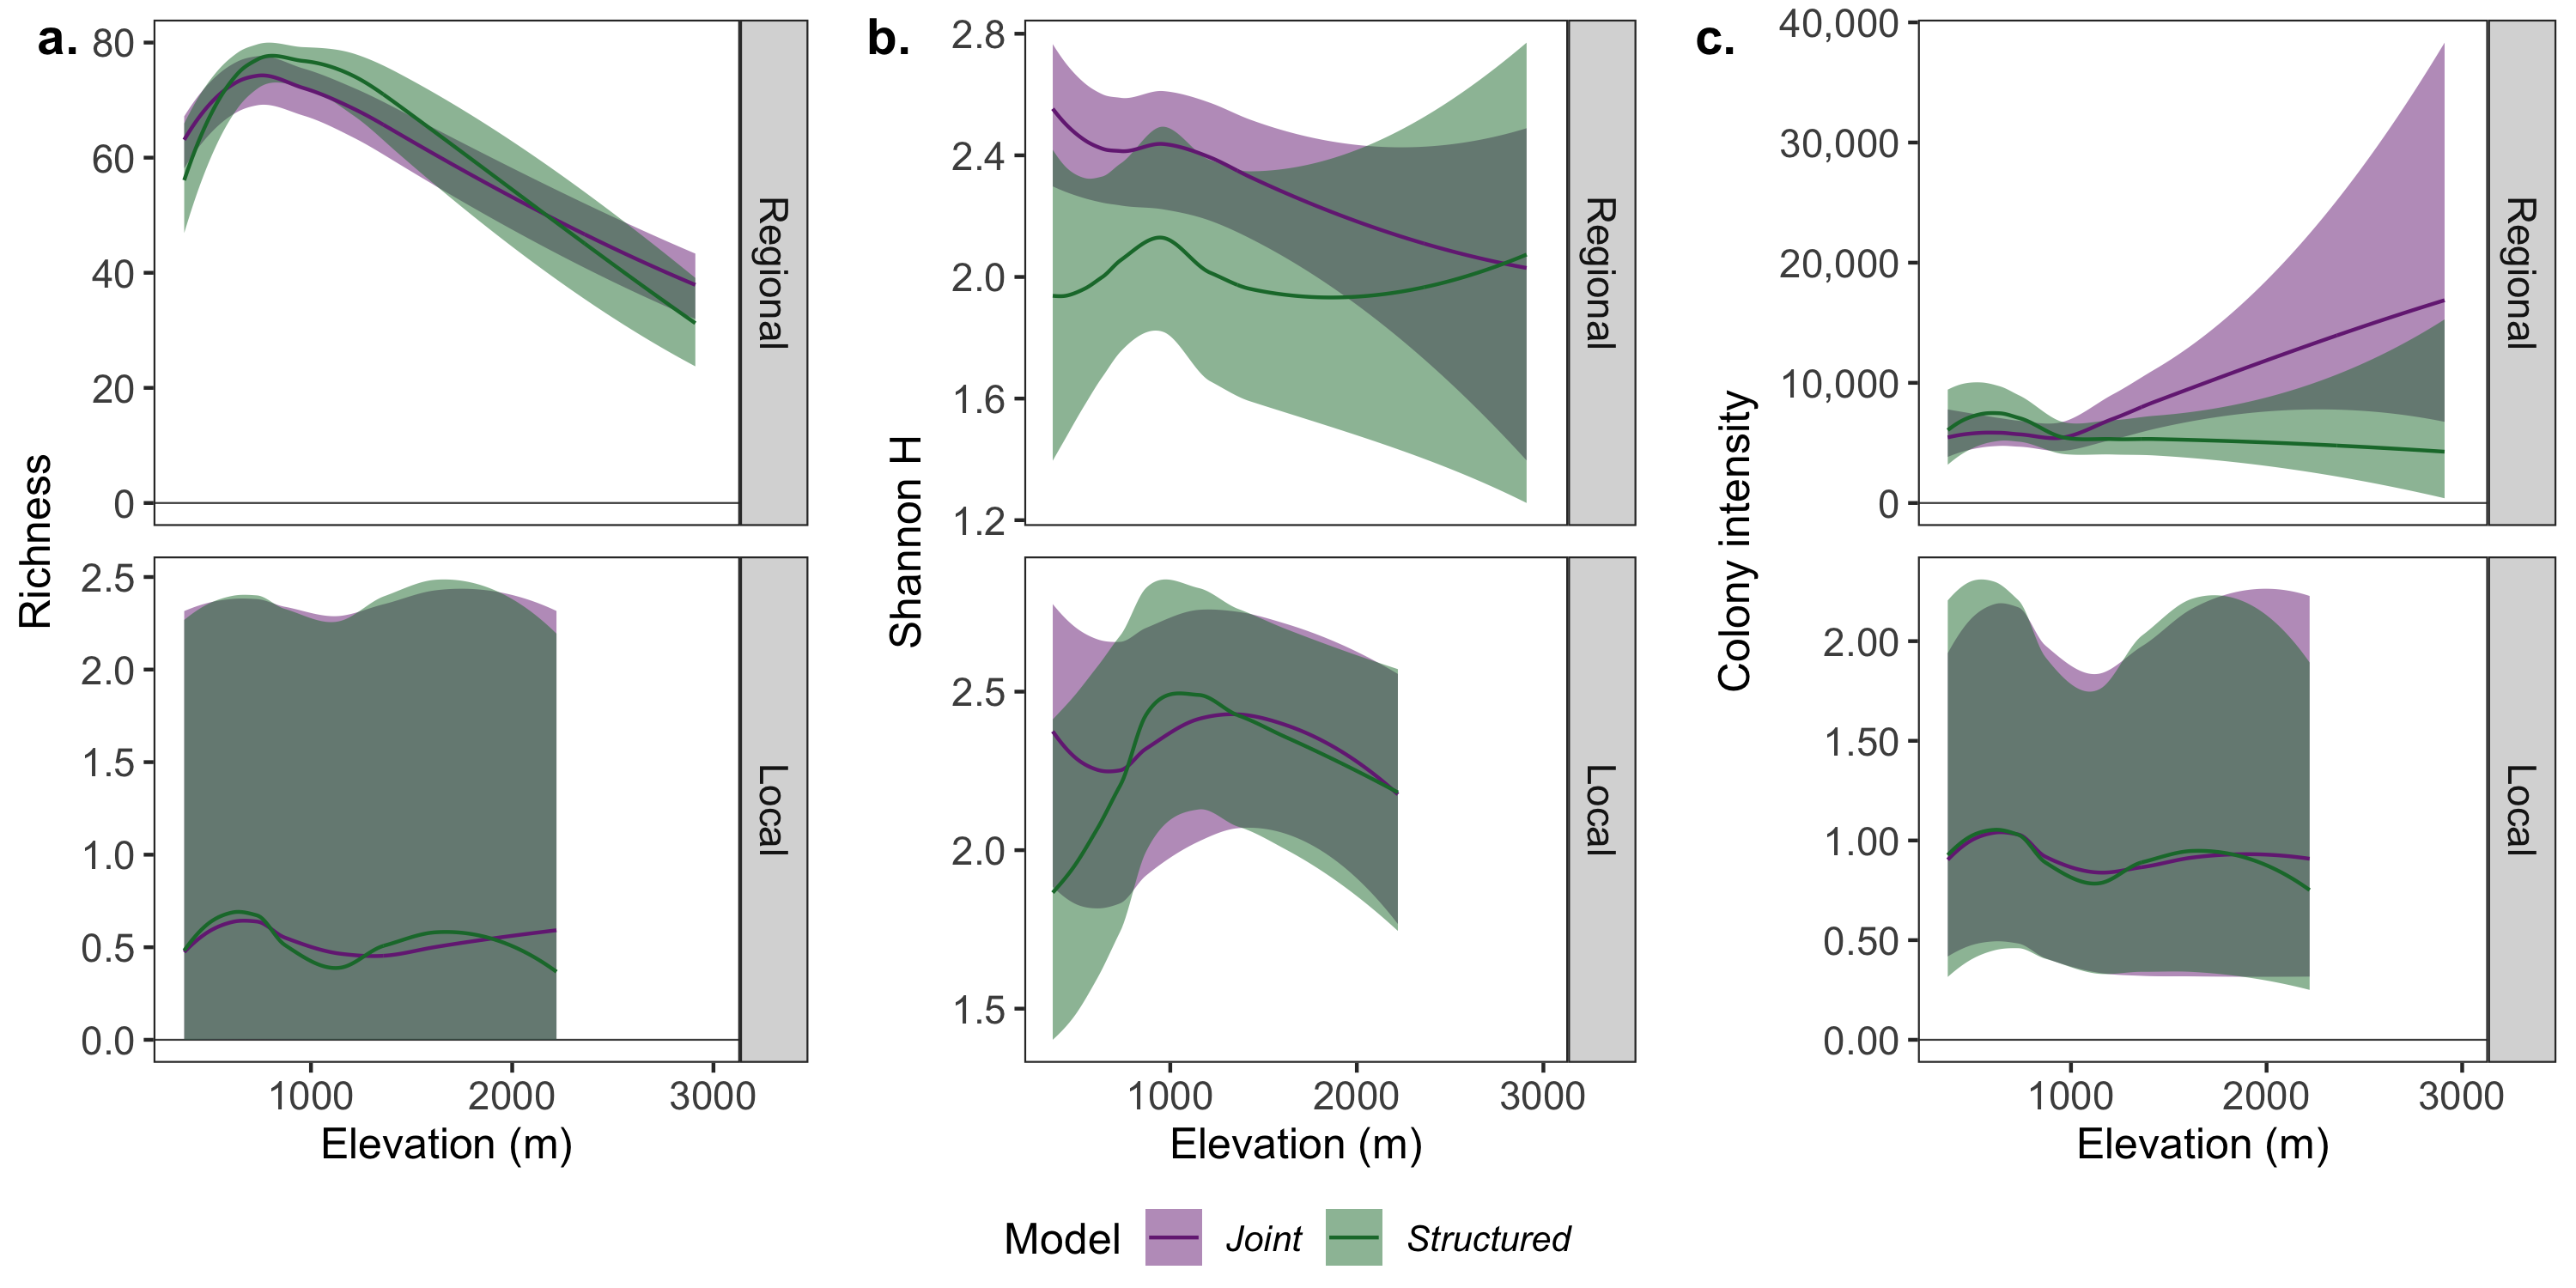
\includegraphics[width=6in]{figs/el_patterns.png}
	\caption{\label{fig:el_patterns} Elevational patterns of posterior distributions at regional and local scales for (a) predicted species richness, (b) predicted Shannon H diversity, and (c) colony intensity. Lines and ribbons are loess lines using the posterior medians and 95\% Highest Density Interval, respectively, for the model using both datasets (Joint: purple) and the model using only the structured abundance data (Structured: green). All metrics were calculated in each sample from the posterior distribution using the predicted species-level colony intensities. }
\end{figure}

\begin{figure}
\centering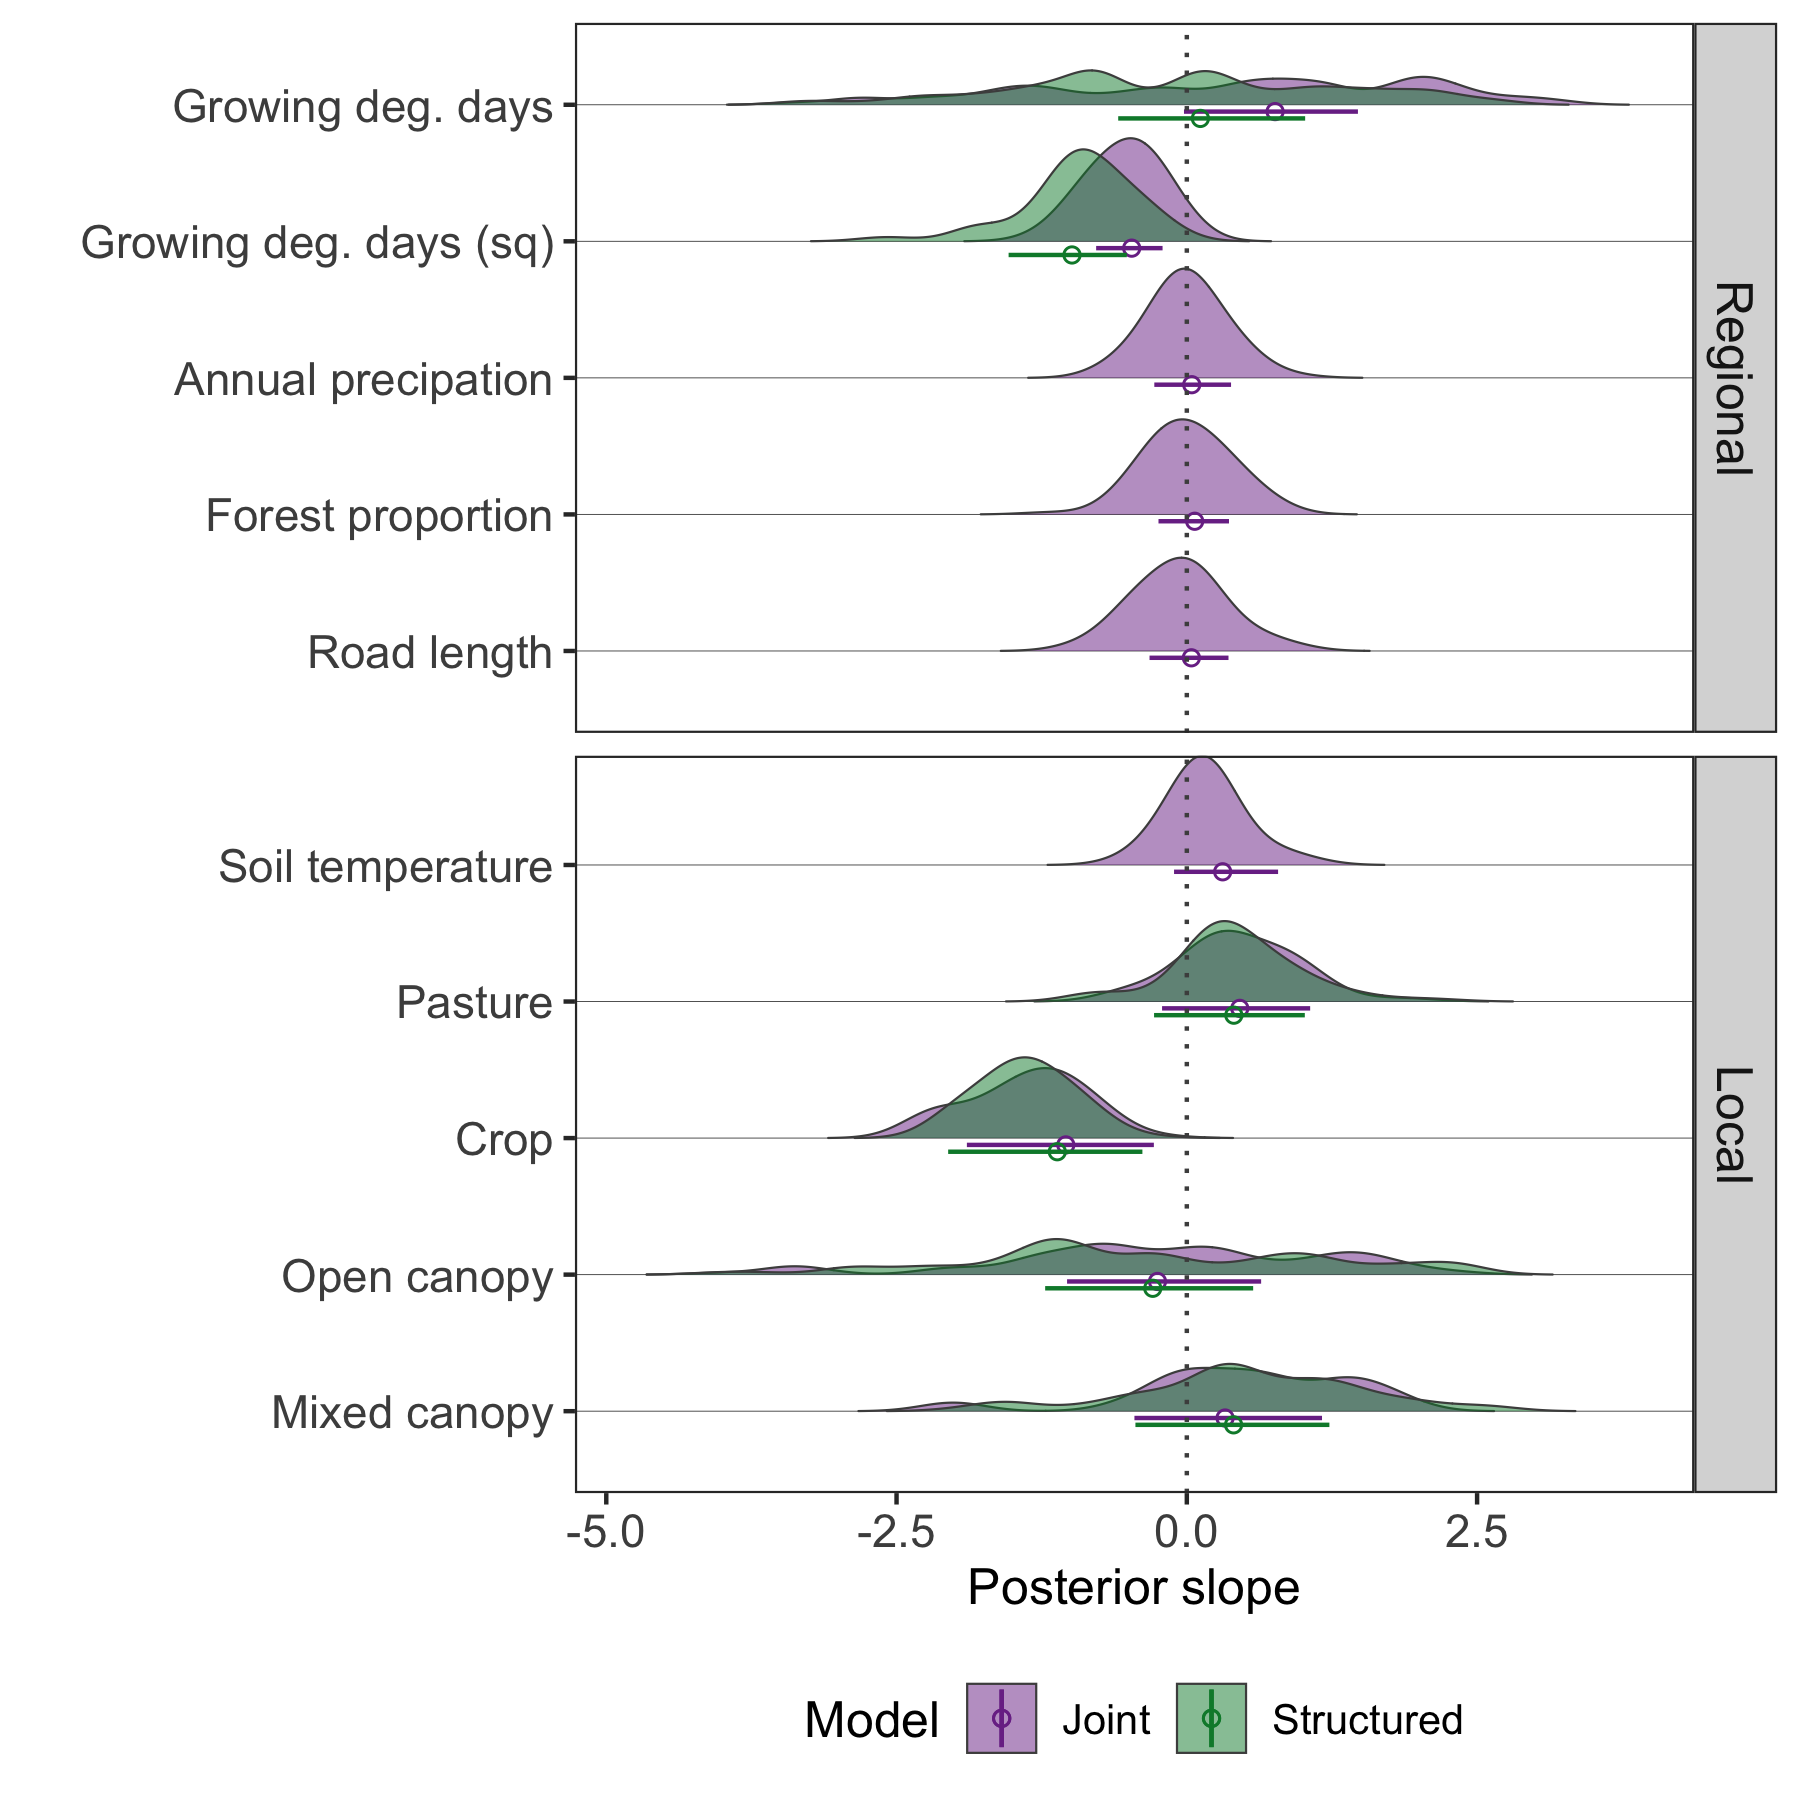
\includegraphics[width=4in]{figs/slope_means.png}
\caption{\label{fig:slope_means} Distribution of species-level responses in optimal models. Density curves represent the distribution of species-level posterior medians for the responses to local and regional variables for the model using both datasets (Joint: purple) and the model using only the abundance data (Structured: green). Points and lines show the posterior median and 95\% Highest Density Interval for the aggregate ($\beta$) responses. }
\end{figure}

\begin{figure}
	\centering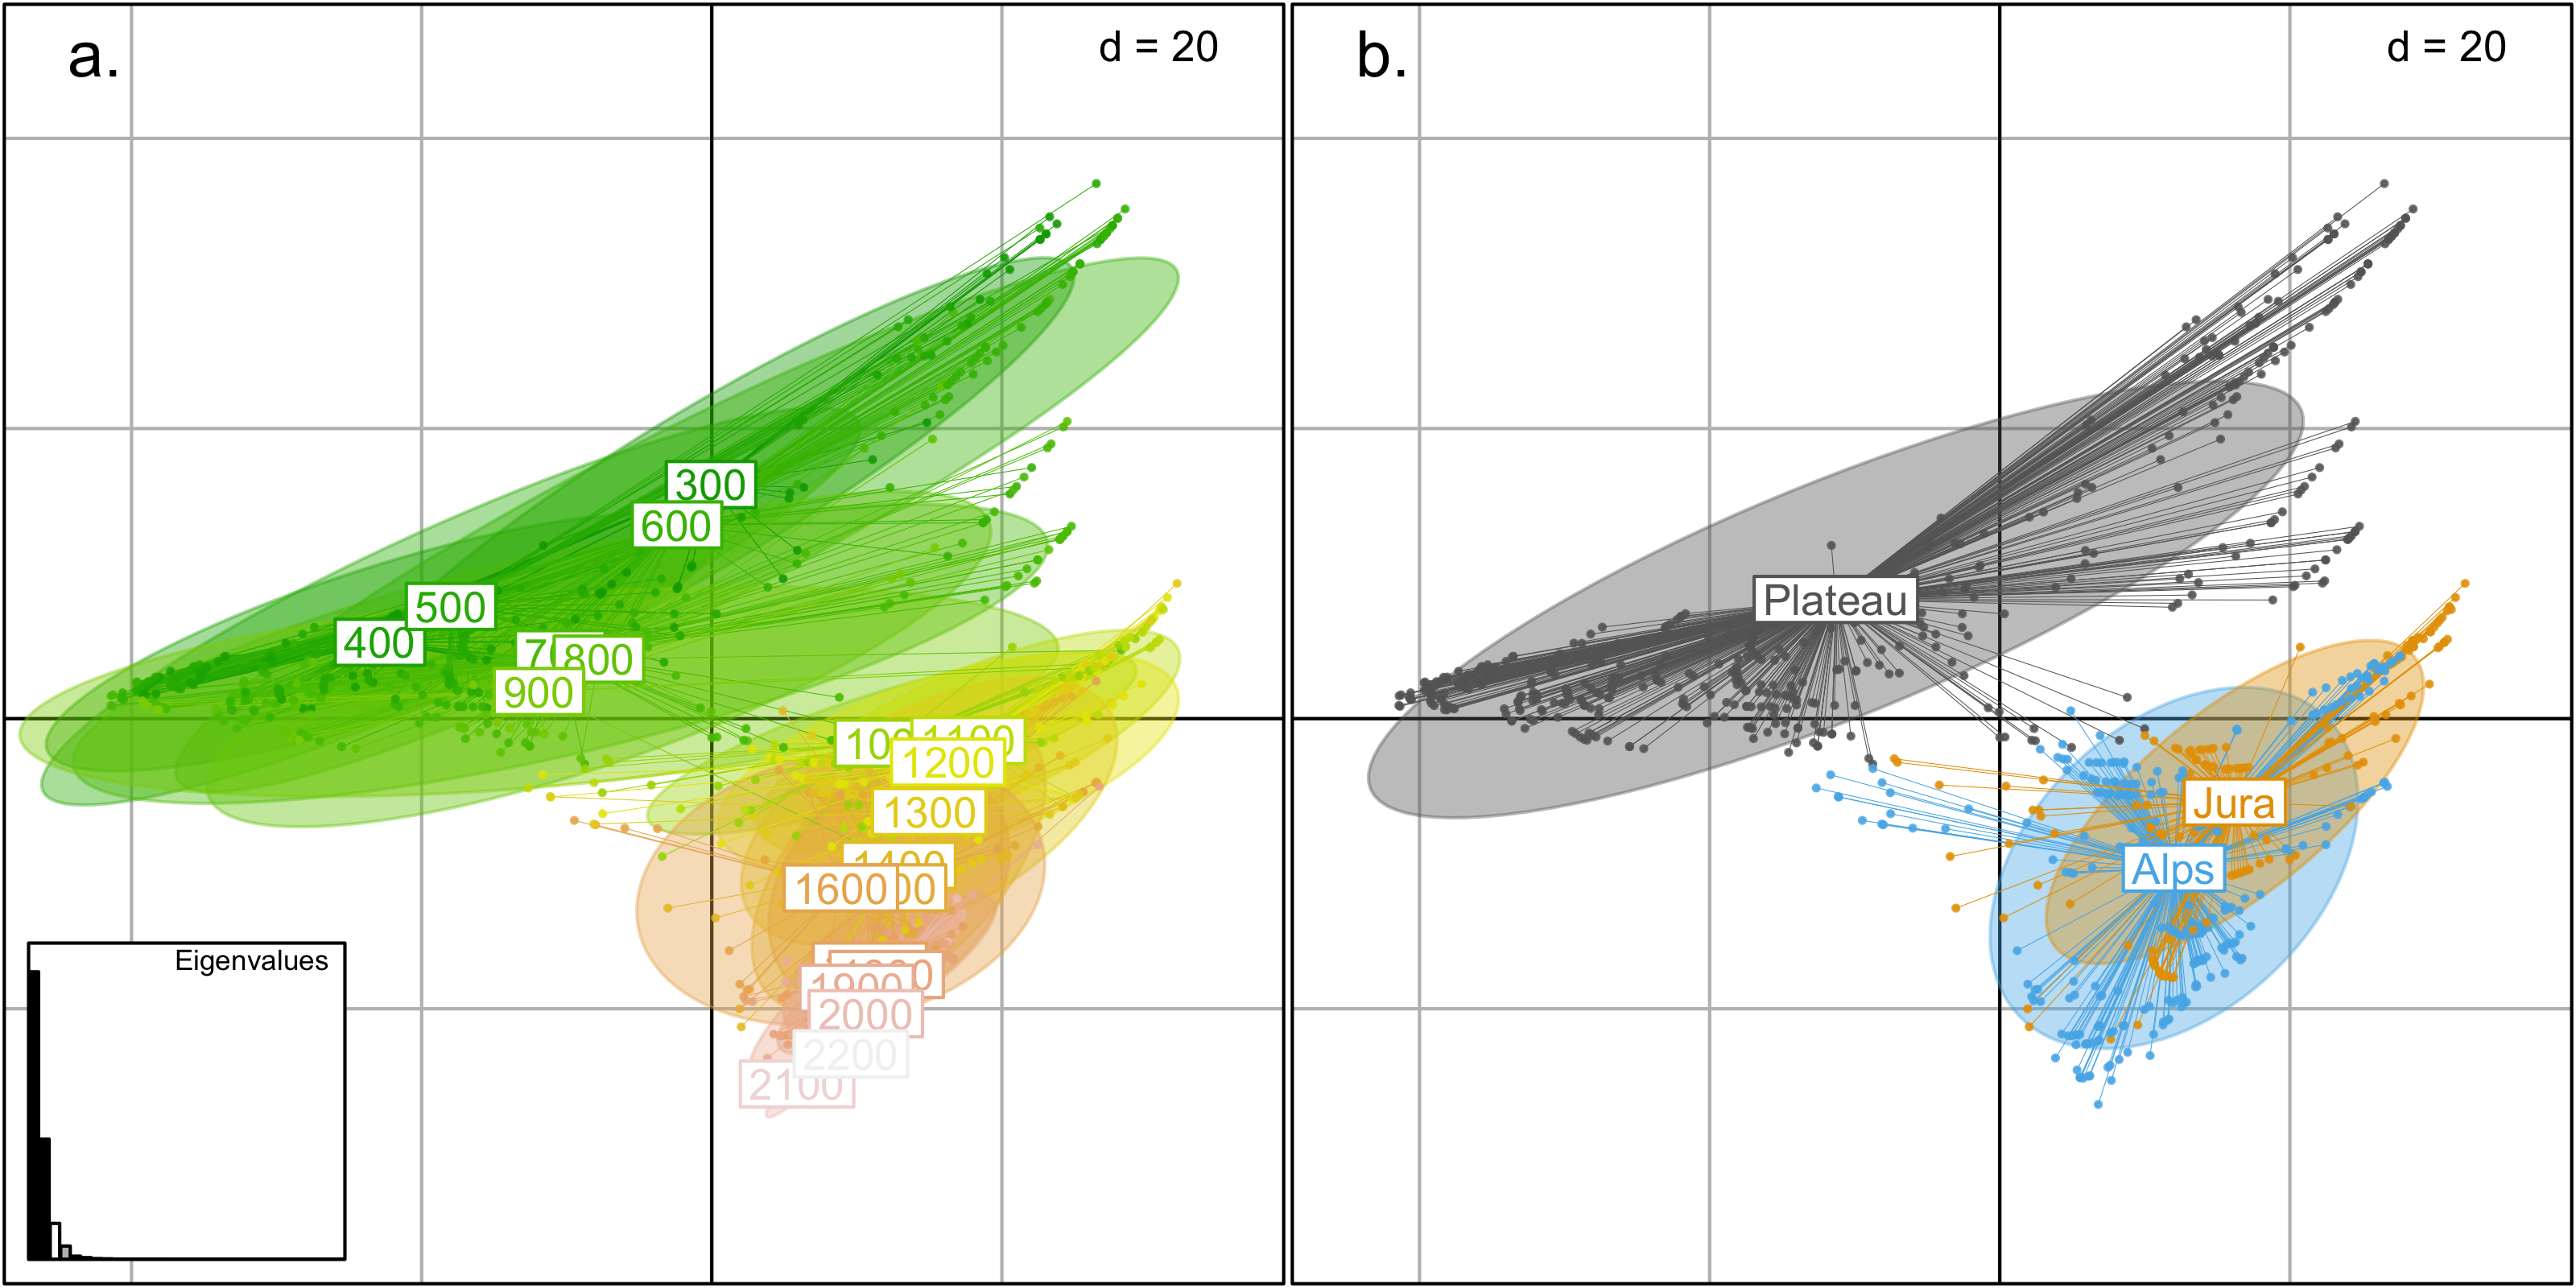
\includegraphics[width=5in]{figs/DPCoA.png}
	\caption{\label{fig:dpcoa} Double principle coordinate analysis (DPCoA) of predicted local communities, with plots colored by (a) elevational bin, and (b) region. The central plateau includes hills from ~300m to ~1000m, with the Jura and the Alps rising steeply in the east and west, respectively. }
\end{figure}

\begin{figure}
	\centering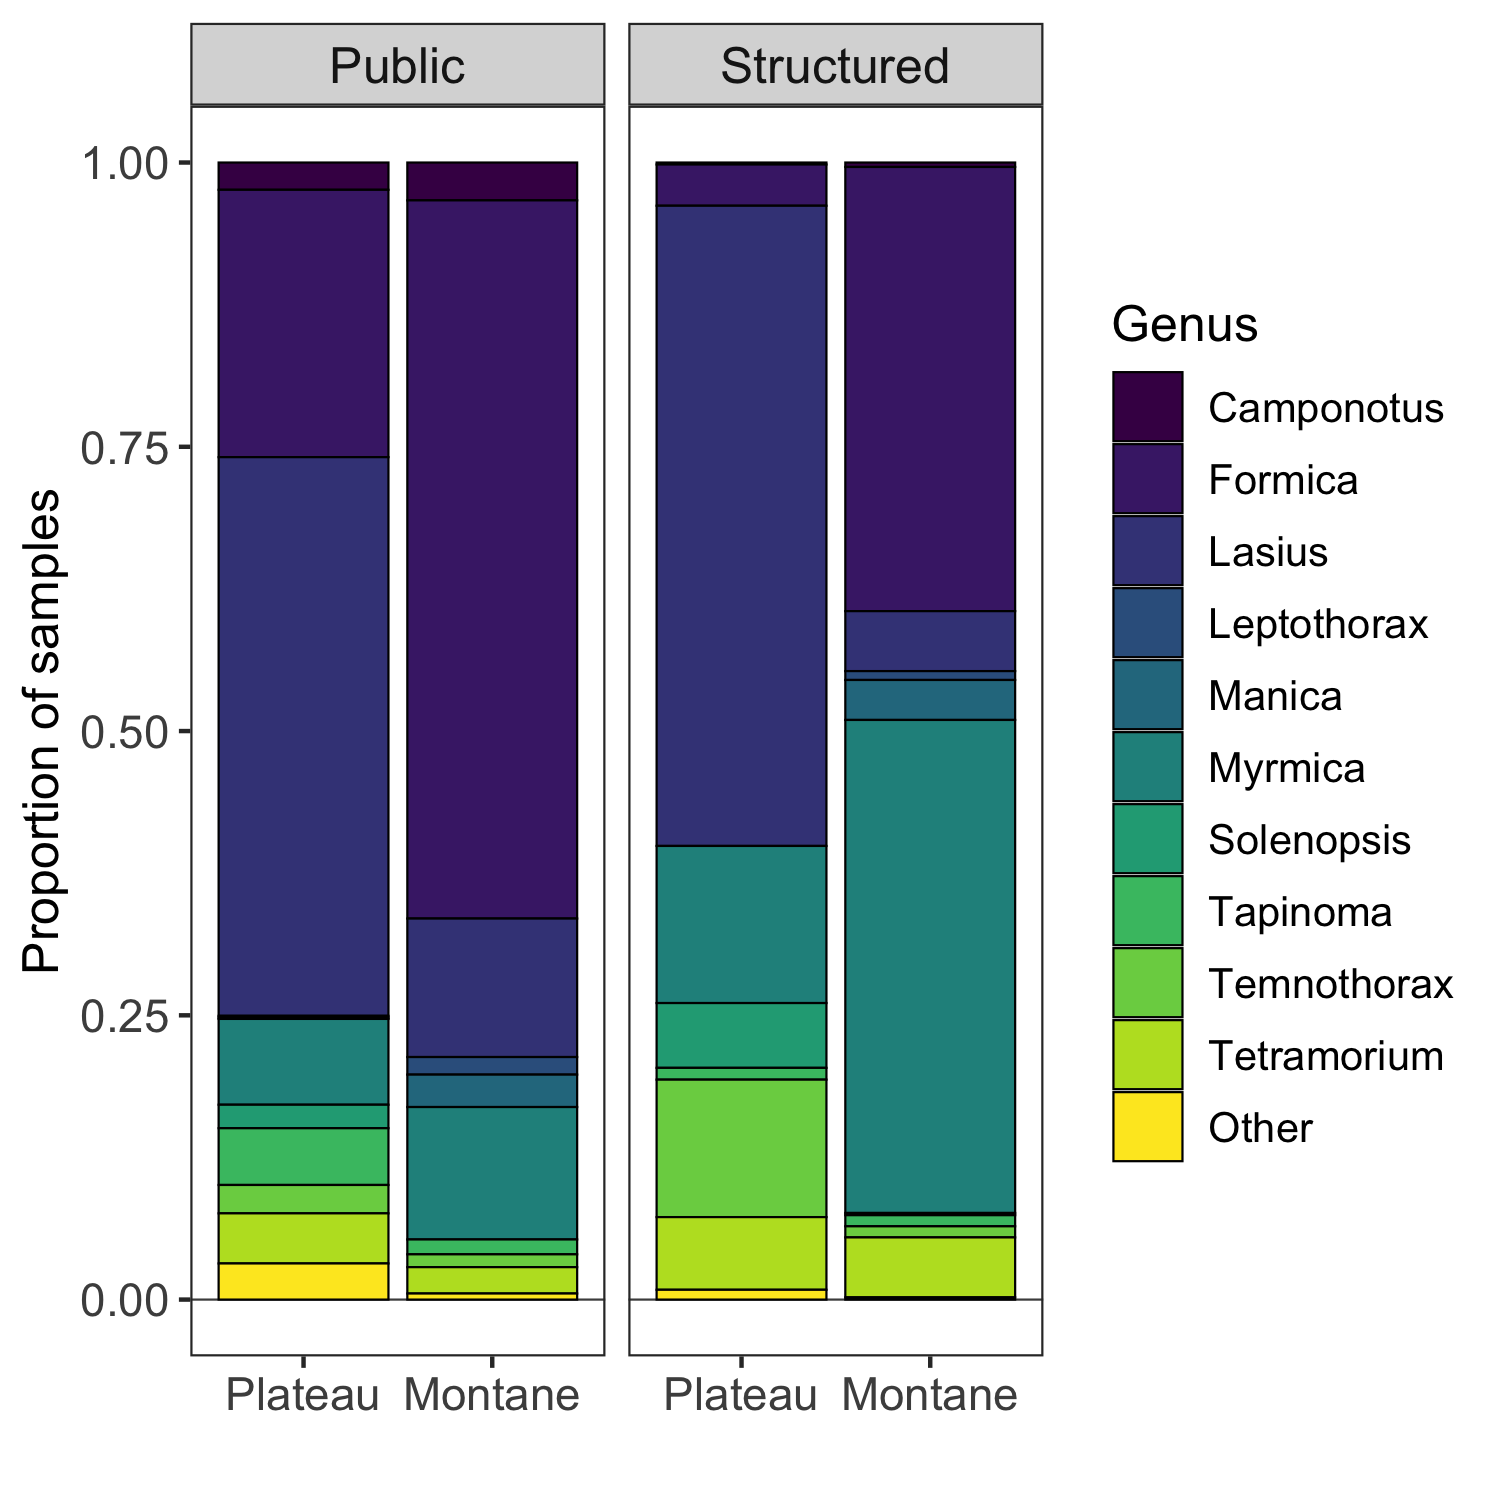
\includegraphics[width=3in]{figs/genus_assemblages.png}
	\caption{\label{fig:genus_assemblages} Relative abundance of genera in the presence-only (public) and abundance (structured) datasets across plateau and montane environments. Only genera that constitute $\geq 1\%$ of at least one subset are shown, with all others indicated as 'Other'.}
\end{figure}

\begin{figure}
\centering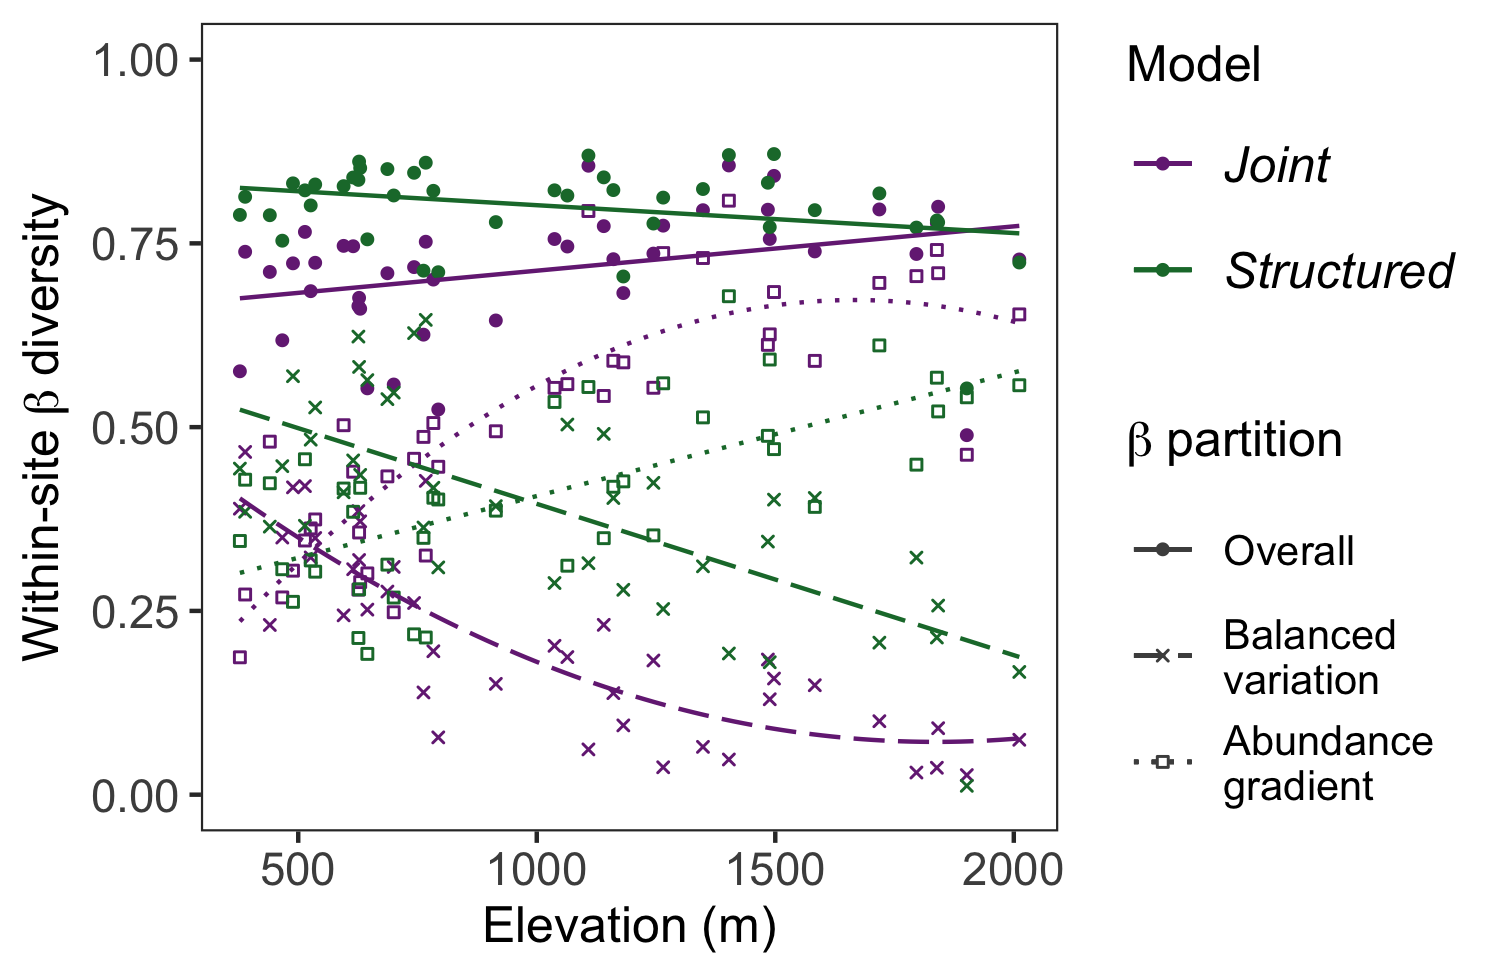
\includegraphics[width=3in]{figs/beta_diversity.png}
\caption{\label{fig:beta_div} Multi-site $\beta$-diversity and its components across elevation. Within each $1 km^2$ site, the species-level colony intensity posterior medians were used to calculate a multi-site $\beta$-diversity index and its components, representing the variation among local plots. 'Balanced variation' represents changes in relative abundance among species, while the 'abundance gradient' partition denotes changes in total abundance.}
\end{figure}

We used simulated data to validate the model, testing versions of the model using only \textbf{W}, only \textbf{Y}, and both \textbf{W} and \textbf{Y}. The model using both datasets performs best at predicting both site-level and plot-level abundances for testing subsets. I don't have any statistics yet, and will need to do full runs to be more confident. It is, of course, unsurprising that the site-level abundance $\Lambda$ is predicted more accurately, as the use of both datasets effectively increases the sample size for estimating the site-level slopes. The more accurate prediction of $\lambda$ is more exciting, since \textbf{W} doesn't directly include any information about it, but rather helps indirectly by improving predictions of $\Lambda$ at each site, which helps to constrain the intercept in the plot-level equation. 




\section{Discussion}
\label{S:4}
% Summary
Discussion goes here.

% Conclusion
Conclusion



\section{Acknowledgments}
Thanks to everyone.



\section{Appendixes}
\textbf{Appendix 1.} Supplementary methods.  

\textbf{Appendix 2.} Model code.

\textbf{Full equations}  
\begin{equation}
Y_{is} \sim Poisson(\lambda_{is}) \\
\end{equation}

\begin{equation}
log(\lambda_{is}) = a_s V_i + log(h\Lambda_{js}) \\
\end{equation}

\begin{equation}
W_{ks} \sim Poisson(\Lambda_{ks}E_kD_s) \\
\end{equation}

\begin{equation}
log(\Lambda_{(j,k)s}) = b_s X_{(j,k)} \\
\end{equation}

\begin{equation}
logit(E_k) = \eta U_k \\
\end{equation}

\begin{equation}
\begin{gathered}
a_s \sim Norm(A_g, \sigma^a) \\
A_g \sim Norm_G(\alpha, \Sigma^A) \\
\end{gathered}
\end{equation}

\begin{equation}
\begin{gathered}
b_s \sim Norm(B_g, \sigma^b) \\
B_g \sim Norm_G(\beta, \Sigma^B) \\
\end{gathered}
\end{equation}



\section{Bibliography}
\bibliography{ms/opfo_diversity}


\end{document}
